\section[Operating System concepts]{Operating System concepts}

\subsection[Multiprogramming]{Multiprogramming}

Multiprogramming defines a computer where it can run serveral programs at the same time. To enable multiprogramming the OS must be capable of managing memory region for processes, scheduling running time for processes, and many more crucial tasks. We will briefly review the two aspect of multiprogramming.

The first aspect is scheduling. Cooperative multitasking, or so called non-preemptive multitasking, is a design for multiprogramming scheduling where it does not limit a process's runtime. A process will actively run until it stops/idles or waits for an I/O operation, whence the operating system will switch context to another process. In contrast with cooperative multitasking, preemptive multitasking limits the process's runtime and initiate a conext switch when the criteria is met. Both approach have been used in many operating systems but cooperative multitasking schema sometimes causes system to hang, thus in most modern operating system (Windows, MacOS, and most Linux distributions), preemptive multitasking schema is chosen.

\begin{figure}
  \centering
  \caption{Preemptive}
  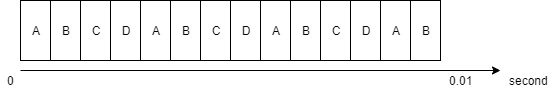
\includegraphics[scale=0.8]{images/preemptive.png}
  \text{4 processes (A, B, C, D) running in a tiny time slot which appears simutaneously to a human}
\end{figure}

The second aspect is memory management. In the early days, memory management was so simple that it would contain the whole process consecutively in memory. However, doing this leads to external fragmentation\footnote{the memory is empty but not fit consecutively for a process}. Then people realize that it is not optimized to contain the whole process in memory because some part of it is unused at a specific point of time. For example, when we have a program with many functions, at one time we only run a few of them. To optimize this, people choose to load only the necessary parts in memory. After many years of optimizing, people have agreed upon splitting a process to equal parts called a \textit{page}. The OS split the physical memory to pages and load process to those pages. When a process needs more space or needs parts that are not on memory, the OS will find an empty/unused page to load in. If there is no empty page, one least use page will be swapped out to disk to make space. The OS tracks what pages a process is using and swap those pages in when the process needs.


So far, we have only discussed processes that have a limited amount of memory, but OS allows programs to have more space by using the paging technique describe above. A process can have a virtual space of addresses with which it can use. Every process running will have a certain amount of \textit{virtual} memory available. Assuming we have a process, that process will have 2GB of memory (from 0 to $2^{32}-1$) and at 0x40000000 is the start of \texttt{.text} section from that process point of view. However the page from \texttt{.code} to \texttt{.code + page\_size} is located in RAM at address 0x60000000 to 0x60000000 + \texttt{page\_size}. The OS has to translate the address from 0x40000000 to 0x60000000 when the process accesses any address in page size from 0x40000000. This is called \textit{address translation}. Although access to a memory section is more complex, by using virtual memory, a process can have more memory. If many processes use the same library, that library would be map over to a virtual section of that process.

\begin{figure}
\centering
\caption{External fragmentation}
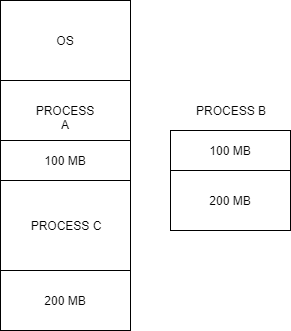
\includegraphics[]{images/external_fragmentation.png}
\end{figure}

\begin{figure}
\centering
\caption{Splitting process}
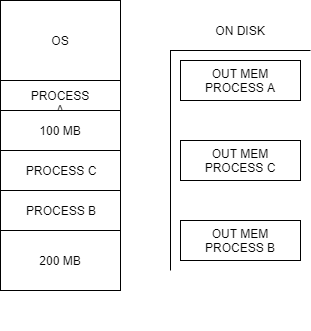
\includegraphics[]{images/splitting_process.png}
\end{figure}

\begin{figure}
\centering
\caption{Splitting process}
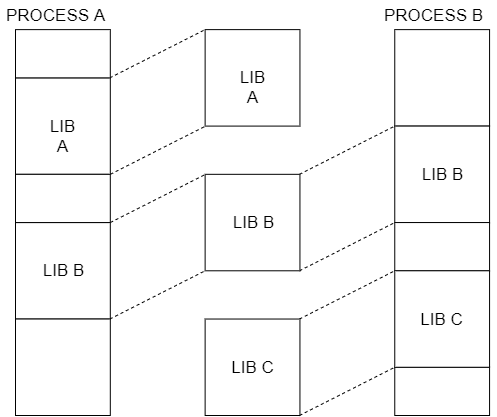
\includegraphics[]{images/use_same_lib.png}
\text{Two processes use the same library (LIB B) and is visible in its own (virtual) address space}
\end{figure}

% TODO: Insert picture

% In modern OS design, people notice that a process not always needed everything to be in memory. Unused parts of a process can be transfered to secondary memory and bring it back to primary one on demand. OS does process spliting base on this theory, split one process into many parts and only load the part that is needed at that time. Spliting of the process can be done in many different ways, but spliting by a constant size is commonly used. This constant size is called a \textit{page}, and by most OS, this amount is 4KB by default. The physical memory is splitted by page also. Every process will have a private address space, called user-space, which one process can write/read and execute. This private address will contain all process's data, including code, data, and heap. All processes have a common shared address space which contains information available system wide, this space is called the kernel-space. Eventhough that all processes share the kernal-space they cannot access this address space due to OS prevention. These two spaces are virtual, the OS mechanism makes processes "think" that they owns a large memory region, while infact memory are splitted and located accross the primary or secondary memory. The picture below contains two processes running, while both of them are loaded the whole memory of the process is not neccessary to be in RAM. Both processes virtualy have a separated memory space, these memory region will be loaded to RAM on demand, and swapped out to disk when unused and the OS needs to load new pages in.

% The design of paging technique is very useful. A process can be splitted to many parts and only loads what is needed, furthurmore, processes that uses the same library can reuse the already loaded one and not neccessary to reload again. Because memory is scattered through the RAM and disks, and each process has a virtual memory space, the OS must keep track of Pages and Pages mapping. When a process access a memory address in the process space, the OS will translate to the physical address lies in RAM.

% \subsection[Multiprocessor]{Multiprocessor}


% \subsection[Threads]{Threads}

